\chapter{Példák}

\section{Sok körzőzés}
\begin{tikzExample}
    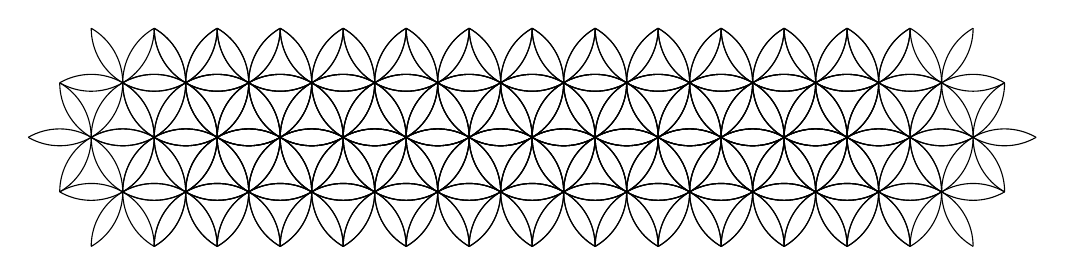
\begin{tikzpicture}[scale=0.8]
        \foreach \i in {0,...,12}
            {
                \draw (\i+0,0) circle (1);
                \draw (\i+0.5,-0.866) arc (0:120:1);
                \draw (\i+1.5,-0.866) arc (0:240:1);
                \draw (\i+-1,-0) arc (60:-60:1);
                \draw (\i+0,-1.732) arc (0:120:1);
                \draw (\i+-1.5,-0.866) arc (-120:120:1);
                \draw (\i+-1,-0) arc (-60:60:1);
                \draw (\i+-1.5,0.866) arc (-120:0:1);
                \draw (\i+0,1.732) arc (120:360:1);
                \draw (\i+0.5,0.866) arc (0:-120:1);
                \draw (\i+0.5,0.866) arc (-60:-180:1);
                \draw (\i+0.5,0.866) arc (120:240:1);
                \draw (\i+0.5,0.866) arc (180:300:1);
                \draw (\i+0.5,-0.866) arc (180:60:1);
                \draw (\i+-1,-1.732) arc (180:60:1);
                \draw (\i+1.5,0.866) arc (120:240:1);
                \draw (\i+0.5, 0.866) arc (0:60:1);
                \draw (\i+0.5, 0.866) arc (240:180:1);
                \draw (\i+0.5, 0.866) arc (240:300:1);
                \draw (\i+0.5, 0.866) arc (120:60:1);
                \draw (\i+0.5, 0.866) arc (180:120:1);
                \draw (\i+0.5, 0.866) arc (300:360:1);
                \draw (\i+-1,-0) arc (0:60:1);
                \draw (\i+-1,-0) arc (240:180:1);
                \draw (\i+-1,-0) arc (60:120:1);
                \draw (\i+-1,-0) arc (300:240:1);
                \draw (\i+-1,-0) arc (120:180:1);
                \draw (\i+-1,-0) arc (360:300:1);
                \draw (\i+0.5, -0.866) arc (180:240:1);
                \draw (\i+0.5, -0.866) arc (60:0:1);
                \draw (\i+0.5, -0.866) arc (120:60:1);
                \draw (\i+0.5, -0.866) arc (240:300:1);
                \draw (\i+0.5, -0.866) arc (120:180:1);
                \draw (\i+0.5, -0.866) arc (360:300:1);
            }
    \end{tikzpicture}
\end{tikzExample}

\section{Sakktábla}
\begin{tikzExample}
    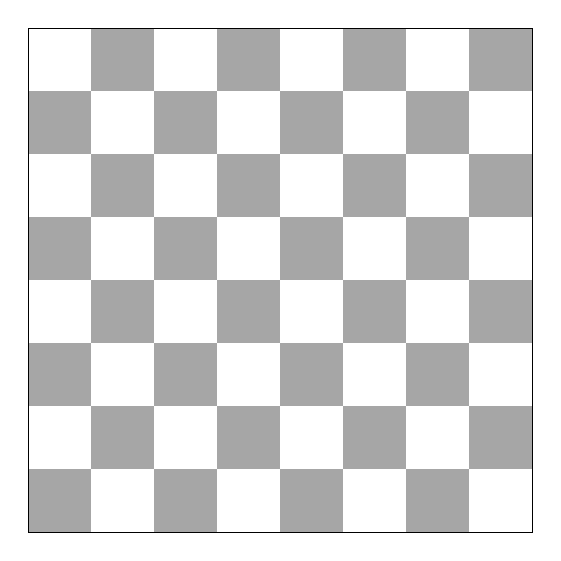
\begin{tikzpicture}[scale=0.8]
        \foreach \i in {1,3,5,7}
        \foreach \j in {1,3,5,7}
        {
            \fill[line width=0.pt, fill=gray,opacity=0.7]
            (\i,\j) -- (\i+1,\j) -- (\i+1,\j+1) -- (\i,\j+1) -- cycle;
            \fill[line width=0.pt, fill=gray,opacity=0.7] (\j,\i) --
            (\j-1,\i) -- (\j-1,\i-1) -- (\j,\i-1) -- cycle;
        }
        \draw (0,0)--(0,8)--(8,8)--(8,0)--cycle;
        \begin{Large}
            \draw (0.5,0.5) node {\bf{\symrook}};
            \draw (1.5,1.5) node {\bf{\symrook}};
            \draw (2.5,2.5) node {\bf{\symrook}};
            \draw (3.5,3.5) node {\bf{\symrook}};
            \draw (4.5,7.5) node {\bf{\symbishop}};
            \draw (5.5,7.5) node {\bf{\symbishop}};
            \draw (6.5,4.5) node {\bf{\symbishop}};
            \draw (7.5,6.5) node {\bf{\symbishop}};
        \end{Large}
    \end{tikzpicture}
\end{tikzExample}

\section{Óxisz szigete}
\begin{tikzExample}
    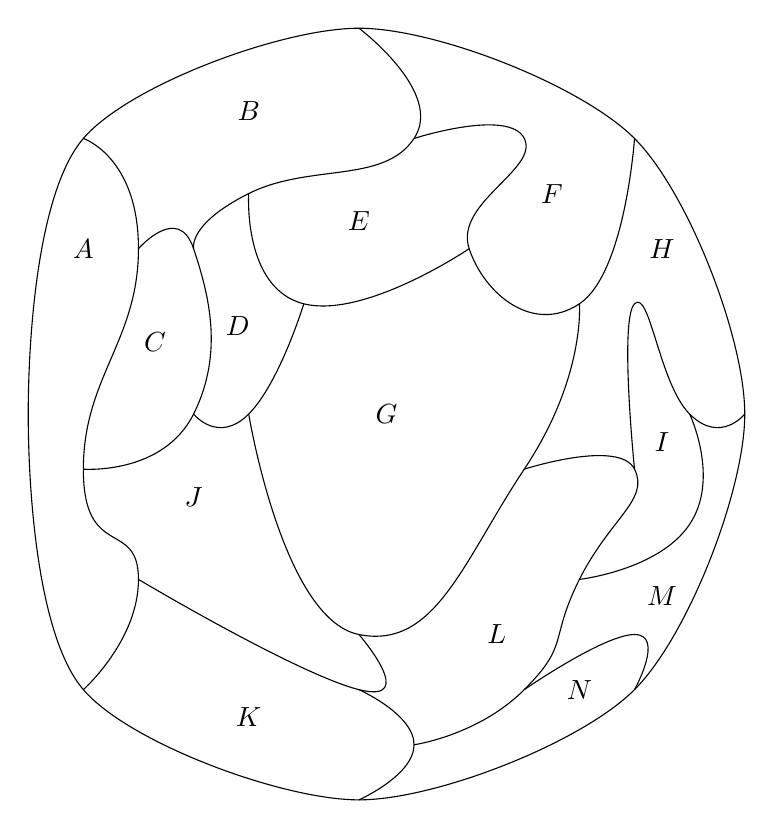
\begin{tikzpicture}[scale = 0.7]
        \draw plot [smooth cycle, tension = 0.5] coordinates {(0,0) (5,-2)
                (10,0) (12,5) (10,10) (5,12) (0,10) (-1,5)};
        \draw plot [smooth, tension = 1] coordinates {(0,10) (1,8) (0,4) (1,2) (0,0)}; %K12 
        \draw plot [smooth, tension = 1] coordinates {(1,8) (2,8) (2,5) (0,4)}; %K13
        \draw plot [smooth, tension = 1] coordinates {(2,8) (3,9) (6,10) (5,12)}; %K3
        \draw plot [smooth, tension = 1] coordinates {(6,10) (8,10) (7,8) (9,7) (10,10)}; %K4 
        \draw plot [smooth, tension = 1] coordinates {(3,9) (4,7) (7,8)}; %K2 
        \draw plot [smooth, tension = 1] coordinates {(4,7) (3,5) (2,5)}; %K14
        \draw plot [smooth, tension = 1] coordinates {(9,7) (8,4) (5,1) (3,5)}; %K1
        \draw plot [smooth, tension = 1] coordinates {(5,1) (5,0) (1,2)}; %K11
        \draw plot [smooth, tension = 1] coordinates {(5,0) (6,-1) (5,-2)}; %K10
        \draw plot [smooth, tension = 1] coordinates {(6,-1) (8,0) (9,2) (10,4) (8,4)}; %K9
        \draw plot [smooth, tension = 1] coordinates {(10,0) (10,1) (8,0)}; %K8
        \draw plot [smooth, tension = 1] coordinates {(10,4) (10,7) (11,5) (12,5)}; %K5
        \draw plot [smooth, tension = 1] coordinates {(11,5) (11,3) (9,2)}; %K6 és K7

        \draw (0,8) node {$A$};
        \draw (3,10.5) node {$B$};
        \draw (1.3,6.3) node {$C$};
        \draw (2.8,6.6) node {$D$};
        \draw (5,8.5) node {$E$};
        \draw (8.5,9) node {$F$};
        \draw (5.5,5) node {$G$};
        \draw (10.5,8) node {$H$};
        \draw (10.5,4.5) node {$I$};
        \draw (2,3.5) node {$J$};
        \draw (3,-0.5) node {$K$};
        \draw (7.5,1) node {$L$};
        \draw (10.5,1.7) node {$M$};
        \draw (9,0) node {$N$};
    \end{tikzpicture}
\end{tikzExample}

\section{Simson-egyenes}
\begin{tikzExample}
    \begin{tikzpicture}[line cap=round,line join=round,>=triangle
            45,x=0.7cm,y=0.7cm]
        \clip(-7,-5.5) rectangle (9,5.5);
        \fill[color=brown,fill=brown,fill opacity=0.1] (-3,-4) -- (3,-4) --
        (-2,4.58) -- cycle;
        \draw(0,0) circle (3.5cm);
        \draw [color=brown] (-3,-4)-- (3,-4);
        \draw [color=brown] (3,-4)-- (-2,4.58);
        \draw [color=brown] (-2,4.58)-- (-3,-4);

        \draw [line width=0.4pt,domain=-7.44:9.29] plot(\x,{(-24-0*\x)/6});
        \draw [line width=0.4pt,domain=-7.44:9.29] plot(\x,{(-5.75--8.58*\x)/-5});
        \draw [line width=0.4pt,domain=-7.44:9.29] plot(\x,{(-21.74-8.58*\x)/-1});

        \draw [line width=1.2pt,dash pattern=on 3pt off 6pt] (4.66,1.8)-- (0.9,-0.39);
        \draw [line width=1.2pt,dash pattern=on 3pt off 6pt] (-2.23,2.61)-- (4.66,1.8);
        \draw [line width=1.2pt,dash pattern=on 3pt off 6pt] (4.66,1.8)-- (4.66,-4);

        \draw [line width=1.6pt,color=red,domain=-7.44:9.29] plot(\x,{(-1.47--3*\x)/-3.13});

        \begin{small}
            \fill (0,0) circle (1.5pt);
            \fill (-3,-4) circle (1.5pt);
            \draw (-3.5,-4.5) node {$A$};
            \fill (3,-4) circle (1.5pt);
            \draw (2.8,-4.5) node {$B$};
            \fill (-2,4.58) circle (1.5pt);
            \draw (-1.4,4.4) node {$C$};
            \fill (4.66,1.8) circle (1.5pt);
            \draw (4.86,2.12) node {$P$};
            \fill (0.9,-0.39) circle (1.5pt);
            \draw (0.6,-0.7) node {$T_A$};
            \fill (-2.23,2.61) circle (1.5pt);
            \draw (-2.7,2.3) node {$T_B$};
            \fill (4.66,-4) circle (1.5pt);
            \draw (4.5,-4.5) node {$T_C$};
        \end{small}
    \end{tikzpicture}
\end{tikzExample}

% \section{Dijkstra-algoritmus, gráfok}
% \begin{tikzExample}
%     \begin{tikzpicture}[scale=1.6]
%         \begin{small}
%             \GraphInit[vstyle=Dijkstra]
%             \Vertex[x=0,y=0,L=$\mathbf{s}$]{A}
%             \Vertex[x=3,y=0,L=$v_1$]{B}
%             \Vertex[x=4,y=1.5,L=$v_2$]{C}
%             \Vertex[x=3,y=3,L=$v_3$]{D}
%             \Vertex[x=0,y=3,L=$v_4$]{E}
%             \Vertex[x=1,y=2,L=$v_5$]{F}
%             \Vertex[x=1,y=1,L=$v_6$]{G}
%             \Vertex[x=2.5,y=1,L=$v_7$]{H}
%             \Vertex[x=2.5,y=2,L=$\mathbf{t}$]{I}
%             \tikzset{EdgeStyle/.style={line width=1.2,-}}
%             \Edge[label=6](A)(B)
%             \Edge[label=5](B)(C)
%             \Edge[label=7](B)(G)
%             \Edge[label=5](C)(D)
%             \Edge[label=4](C)(H)
%             \Edge[label=6](D)(F)
%             \Edge[label=3](D)(I)
%             \tikzset{EdgeStyle/.style={line width=1.6,blue,-}}
%             \Edge[label=5](A)(E)
%             \Edge[label=4](E)(F)
%             \Edge[label=2](F)(G)
%             \Edge[label=3](G)(H)
%             \Edge[label=2](H)(I)
%         \end{small}
%     \end{tikzpicture}
% \end{tikzExample}

\section{Komplex egységgyökök}
\subsection{Harmadik egységgyökök}
\begin{tikzExample}
    \def\n{3}
    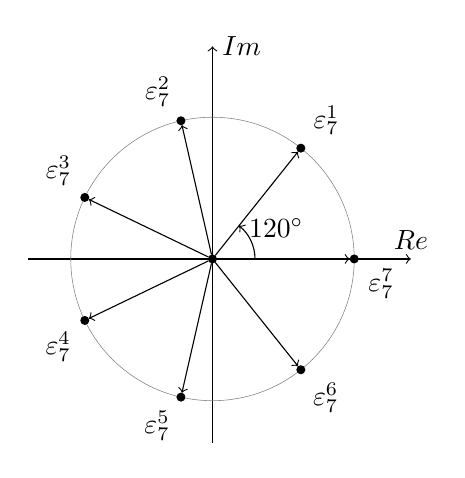
\begin{tikzpicture}[scale=1.8,
        dot/.style={draw,fill,circle,inner sep=1pt}]

        \draw[->] (-1.3,0) -- (1.4,0) node[above] {$Re$};
        \draw[->] (0,-1.3) -- (0,1.5) node[right] {$Im$};
        \draw[help lines] (0,0) circle (1);

        \node[dot] (O) at (0,0) {};
        \foreach \i in {1,...,\n} 
        {
            \node[dot,label={\i*360/\n-(\i==\n)*45:$\varepsilon_{\n}^{\i}$}] (w\i) 
                at (\i*360/\n:1) {};
            \draw[->] (O) -- (w\i);
        }
        \draw[->] (0:.3) arc (0:360/\n:.3);
        \node at (360/\n/2:.5) {$120^\circ$};
    \end{tikzpicture}
\end{tikzExample}

\subsection{Hetedik egységgyökök}
\begin{tikzExample}
    \def\n{7}
    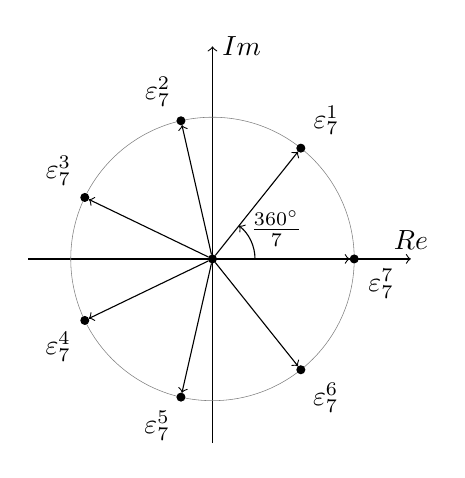
\begin{tikzpicture}[scale=1.8, dot/.style={draw,fill,circle,inner sep=1pt}]

        \draw[->] (-1.3,0) -- (1.4,0) node[above] {$Re$};
        \draw[->] (0,-1.3) -- (0,1.5) node[right] {$Im$};
        \draw[help lines] (0,0) circle (1);

        \node[dot] (O) at (0,0) {};
        \foreach \i in {1,...,\n} {
                \node[dot,label={\i*360/\n-(\i==\n)*45:$\varepsilon_{\n}^{\i}$}] (w\i)
                at (\i*360/\n:1) {};
                \draw[->] (O) -- (w\i);
        }
        \draw[->] (0:.3) arc (0:360/\n:.3);
        \node at (360/\n/2:.5) {$\frac{360^\circ}{\n}$};
    \end{tikzpicture}
\end{tikzExample}

\section{Trigonometrikus függvények}
\begin{tikzExample}
    \definecolor{dgreen}{rgb}{0,0.4,0}
    \begin{tikzpicture}[line cap=round,line join=round,>=triangle
            45,x=1.0cm,y=1.0cm]
        \draw [color=gray,dash pattern=on 2pt off 2pt,
            xstep=1.5707963267948966cm,ystep=1.0cm] (-3.89,-2.97) grid (9.33,2.94);
        \draw[->,color=black] (-3.89,0) -- (9.33,0);
        \draw[shift={(-3.14,0)},color=black] (0pt,2pt) -- (0pt,-2pt)
        node[below] {\footnotesize $-\pi$};
        \draw[shift={(-1.57,0)},color=black] (0pt,2pt) -- (0pt,-2pt)
        node[below] {\scriptsize $-\pi/2$};
        \draw[shift={(1.57,0)},color=black] (0pt,2pt) -- (0pt,-2pt) node[below]
        {\footnotesize $\frac{\pi}{2}$};
        \draw[shift={(pi,0)},color=black] (0pt,2pt) -- (0pt,-2pt) node[below]
        {\footnotesize $\pi$};
        \draw[shift={(4.71,0)},color=black] (0pt,2pt) -- (0pt,-2pt) node[below]
        {\footnotesize $\frac32 \pi$};
        \draw[shift={(6.28,0)},color=black] (0pt,2pt) -- (0pt,-2pt) node[below]
        {\footnotesize $2\pi$};
        \draw[shift={(7.85,0)},color=black] (0pt,2pt) -- (0pt,-2pt) node[below]
        {\footnotesize $\frac52 \pi$};

        \draw[->,color=black] (0,-2.97) -- (0,2.94);
        \foreach \y in {-2,-1,1,2}
            \draw[shift={(0,\y)},color=black] (2pt,0pt) -- (-2pt,0pt) node[left] {\footnotesize $\y$};
        \draw[color=black] (0pt,-10pt) node[right] {\footnotesize $0$};

        \clip(-3.89,-2.97) rectangle (9.33,2.94);
        \draw[line width=1.5pt,dash pattern=on 2pt off 2pt,color=blue,
            smooth,samples=100,domain=-3.8859126567579696:9.331288233648893]
        plot(\x,{sin(((\x))*180/pi)});
        \draw[line width=1.5pt,dash pattern=on 1pt off 2pt on 5pt off
            4pt,color=red,
            smooth,samples=100,domain=-3.8859126567579696:9.331288233648893]
        plot(\x,{cos(((\x))*180/pi)});
        \draw[line width=1.2pt, color=dgreen,
            smooth,samples=100,domain=-1.56-pi:1.56-pi] plot
        (\x,{sin(((\x))*180/pi)/cos(((\x))*180/pi)});
        \draw[line width=1.2pt, color=dgreen,
            smooth,samples=100,domain=-1.56:1.56] plot
        (\x,{sin(((\x))*180/pi)/cos(((\x))*180/pi)});
        \draw[line width=1.2pt, color=dgreen,
            smooth,samples=100,domain=-1.56+pi:1.56+pi] plot
        (\x,{sin(((\x))*180/pi)/cos(((\x))*180/pi)});
        \draw[line width=1.2pt, color=dgreen,
            smooth,samples=100,domain=-1.56+pi+pi:1.56+pi+pi] plot
        (\x,{sin(((\x))*180/pi)/cos(((\x))*180/pi)});
        \draw[line width=1.2pt, color=dgreen,
            smooth,samples=100,domain=-1.56+pi+pi+pi:1.56+pi+pi+pi] plot
        (\x,{sin(((\x))*180/pi)/cos(((\x))*180/pi)});
        \begin{scriptsize}
        \end{scriptsize}
    \end{tikzpicture}
$\color{blue}{f(x) = \sin x} \hspace{2 cm} \color{red}{g(x) = \cos x } \hspace{2 cm} \color{dgreen}{h(x) = \mathrm{tg}x} $
\end{tikzExample}

\section{Nyolcszög, lyukkal}
\begin{tikzExample}
    \newcommand*\st{1.414142135}
    \begin{tikzpicture}[scale=2, line cap=round]
        \fill[gray, pattern = horizontal lines] 
            (-1,-1)--(0,-\st)--(1,-1)--(\st,0)--(1,1)--(0,\st)--(-1,1)--(-\st,0)--cycle;
        \fill[white] 
            (-1,-1)--(0,-2+\st)--(1,-1)--(2-\st,0)--(1,1)--(0,2-\st)--(-1,1)--(-2+\st,0)--cycle;
        \fill[gray, pattern = vertical lines] 
            (-1,-1)--(0,-2+\st)--(1,-1)--(2-\st,0)--(1,1)--(0,2-\st)--(-1,1)--(-2+\st,0)--cycle;
        \fill[white] 
            (0,2-\st)--(2-\st,0)--(0,\st-2)--(\st-2,0)--cycle;

        \draw[line width=2] (-1,-1)--(0,-\st)--(1,-1)--(\st,0)--(1,1)--(0,\st)--(-1,1)--(-\st,0)--cycle;
        \draw[line width=2] (-1,-1)--(0,-2+\st)--(1,-1)--(2-\st,0)--(1,1)--(0,2-\st)--(-1,1)--(-2+\st,0)--cycle;
        \draw[line width=1.5, dashed] (0,2-\st)--(2-\st,0)--(0,\st-2)--(\st-2,0)--cycle;

        \draw[line width=1.5, dashed] (0,2-\st) -- (0,\st);
        \draw[line width=1.5, dashed] (2-\st,0) -- (\st,0);
        \draw[line width=1.5, dashed] (0,-2+\st) -- (0,-\st);
        \draw[line width=1.5, dashed] (-2+\st,0) -- (-\st,0);
    \end{tikzpicture}
\end{tikzExample}

\section{KöMaL B.5131.}
\begin{tikzExample}
    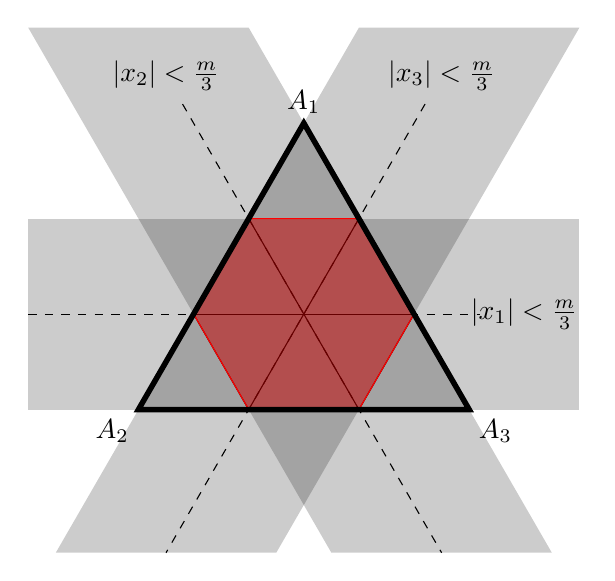
\begin{tikzpicture}[yscale=1.732,scale=0.7]
        \draw[dashed] (-5,0) -- (3.2,0);
        \draw[dashed] (2.2,2.2) -- (-2.5,-2.5);
        \draw[dashed] (-2.2,2.2) -- (2.5,-2.5);

        \draw (-2,0)--(2,0); \draw (-1,1)--(1,1);
        \draw (-1,-1)--(1,1); \draw (1,-1)--(2,0);
        \draw (1,-1)--(-1,1); \draw (-1,-1)--(-2,0);

        \fill[opacity=0.2] (-5,-1)--(5,-1)--(5,1)--(-5,1)--cycle;
        \fill[opacity=0.2] (-1,3)--(-5,3)--(0.5,-2.5)--(4.5,-2.5)--cycle;
        \fill[opacity=0.2] (1,3)--(5,3)--(-0.5,-2.5)--(-4.5,-2.5)--cycle;

        \filldraw[red, fill opacity=0.4] (-1,-1)--(1,-1)--(2,0)--(1,1)--(-1,1)--(-2,0)--cycle;

        \draw[line width=2] (-3,-1)--(3,-1)--(0,2)--cycle;
        \draw (0,2) node [above] {$A_1$};
        \draw (-3,-1) node [below left] {$A_2$};
        \draw (3,-1) node [below right] {$A_3$};

        \draw (4,0) node {$|x_1| < \frac{m}3$};
        \draw (2.5,2.5) node {$|x_3| < \frac{m}3$};
        \draw (-2.5,2.5) node {$|x_2| < \frac{m}3$};
    \end{tikzpicture}
\end{tikzExample}

\section{KöMaL B.5186.}
\begin{tikzExample}
    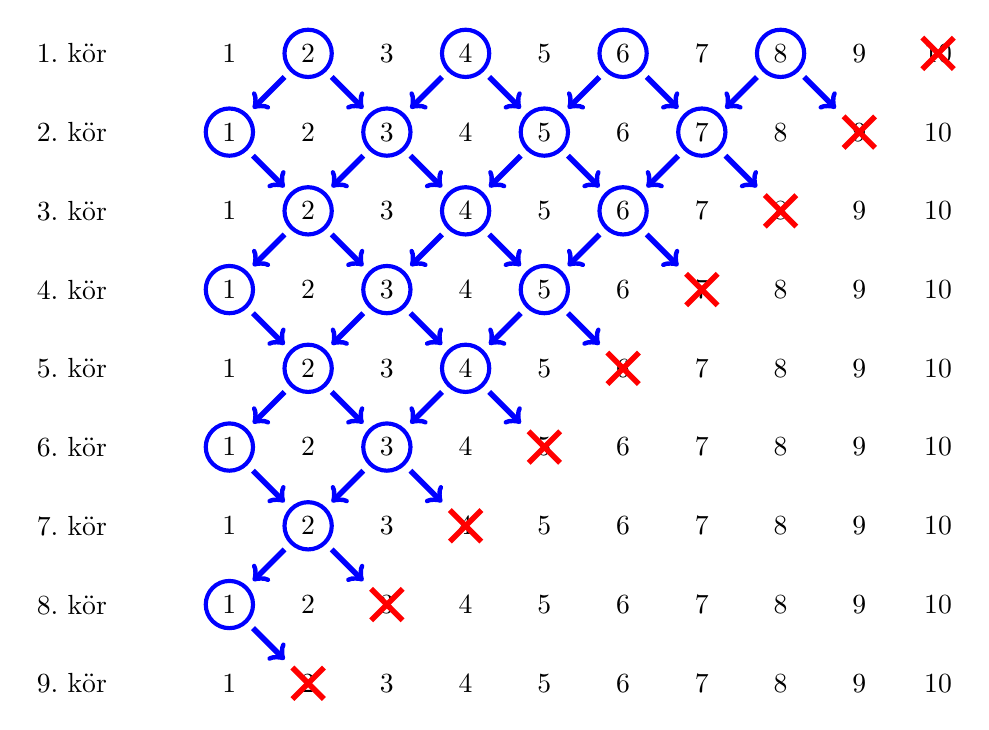
\begin{tikzpicture}
        \foreach \y in {2,...,10}
        \foreach \x in {1,...,10}
        {
            \draw (\x,\y) node {$\x$};
        }

        \foreach \y in {1,...,9}    \draw (-1, 11-\y) node {$\y$.~kör};

        \foreach \y in {2,...,10}
        {
            \draw[red,line width=2] (\y-0.2, \y-0.2) -- (\y+0.2, \y+0.2);
            \draw[red,line width=2] (\y-0.2, \y+0.2) -- (\y+0.2, \y-0.2);
        }

        \foreach \y in {2,3,4,5}
        \foreach \x in {2,...,\y}
        {
            \draw[blue,line width=1.5] (2*\x-2,2*\y) circle (0.3);
            \draw[blue,line width=1.5] (2*\x-3,2*\y-1) circle (0.3);
            \draw[blue,line width=2,->] (2*\x-2.3,2*\y-0.3) -- (2*\x-2.7,2*\y-0.7);
            \draw[blue,line width=2,->] (2*\x-1.7,2*\y-0.3) -- (2*\x-1.3,2*\y-0.7);
            \draw[blue,line width=2,->] (2*\x-2.7,2*\y-1.3) -- (2*\x-2.3,2*\y-1.7);
        }

        \foreach \y in {3,4,5}
        \foreach \x in {3,...,\y}
            \draw[blue,line width=2,->] (2*\x-3.3,2*\y-1.3)-- (2*\x-3.7,2*\y-1.7);
    \end{tikzpicture}
\end{tikzExample}

% \section{KöMaL B.5227.}
% \begin{tikzExample}
%     \begin{tikzpicture}[scale = 1]

%         \draw (0,0) -- (-2,-1);
%         \draw (0,0) -- (2,-1);

%         \draw (-3,-2) -- (-2,-1)--(-1,-2);
%         \draw (3,-2) -- (2,-1)--(1,-2);

%         \draw (-3.5,-3) -- (-3,-2)--(-2.5,-3);
%         \draw (-1.5,-3) -- (-1,-2)--(-0.5,-3);
%         \draw (3.5,-3) -- (3,-2)--(2.5,-3);
%         \draw (1.5,-3) -- (1,-2)--(0.5,-3);

%         \fill (0,0) circle (0.1);
%         \fill (2,-1) circle (0.1);
%         \fill (-2,-1) circle (0.1);
%         \fill (1,-2) circle (0.1);
%         \fill (3,-2) circle (0.1);
%         \fill (-1,-2) circle (0.1);
%         \fill (-3,-2) circle (0.1);
%         \foreach \i in {0,...,7}
%             \fill (\i-3.5,-3) circle (0.1);

%         \draw (5,0) node {$n=3$};
%         \draw (6,-1) node {$V_n = 2^4-1 = 15$};
%         \draw (6.3,-2) node {$S_n = 2^4-4-1 = 4$};
%         \draw (6,-3) node {$k = 2^3+3 = 11$};

%         \draw[blue] (1,-2.6) circle (1);

%         \draw[blue] (-1.5,-3) circle (0.4);

%         \draw[red,dashed, line width=1.5] (0,0.3) -- (2.2,-0.8) --
%         (3.2,-1.9)--(3.8,-3.2)--(3.4,-3.2)--(3,-2.4) -- (2.7,-3.2)-- (2.2,-3.2)
%         --(2.8,-2) --(1.7,-1.1) -- (0,-0.3)--(-1.6,-1) -- (-0.7,-2) --
%         (-0.2,-3.2)--(-0.7,-3.2)--(-1.3,-2)--(-2,-1.2) -- (-2.8,-2) --

%         (-2.2,-3.2)--(-2.7,-3.2)--(-3,-2.4)--(-3.4,-3.2)--(-3.8,-3.2)--(-3.2,-1.9)--(-2.2,-0.8)--cycle;

%         \begin{Large}
%             \draw[red] (-2,0) node {$G$};
%         \end{Large}

%     \end{tikzpicture}
% \end{tikzExample}